\chapter{Introduction}
\begin{chapterAbstract}{Overview}
	This chapter presents the fundamental concepts of a fuzzy system. It reviews few of the existing fuzzy logic controller designs reported in the literature and analyzes their implementation techniques. This chapter also address the issues of reconfigurability and generality of the existing fuzzy system designs, thereby lay the foundation of this research work and its contribution. 
	
\end{chapterAbstract}
\clearpage
~\\
``We human beings, live in a very imprecise world. A world where our perception of reality are far more important than actual reality.''

\noindent{\bfseries\large\hfill Daniel Keys Moran}
\\
~\\
~\par
It is well known that a human mind efficiently utilizes the modes of imprecision and uncertainty to solve everyday problems. It is this tolerance of imprecision, uncertainty, and approximation that helps human being make informative decisions and enforce reasoning with ease and in a short time. It is true that precision and certainty has ensured that mankind is able to fire precision laser over a long distance, build powerful processors with trillions of transistors, developed terra\hyp{}pixel imaging devices, focus microscopic beams of electron to capture minute details in nanometer scale, and accomplish many more unimaginable achievement in science and technology. However, requiring precision in engineering problems incurs a high cost and long lead time in development. Prof. Lotfi Askar Zadeh described the power of uncertainty and approximate reasoning over hard computing by illustrating how a human mind work while \textit{parking a vehicle}\cite{Zadeh1993}. T. Ross took the instance of \textit{traveling salesman} problem to exemplify similar point \cite{Ross2010}. It is, therefore, important for any scientist or engineer to contemplate the requirement for approximate reasoning and imprecision while considering fuzzy logic to solve a problem. The prime desideratum is {``how much imprecision can the system tolerate''}.

\section{Introduction to Fuzzy Logic Systems}

Lotfi Askar Zadeh in 1965 \cite{zadeh1965fuzzy} proposed fuzzy sets and described it as ``a class of objects with a continuum of grades of membership. Such a set is characterized by a membership function that assigns to each object a grade of membership ranging from zero to one.'' All fuzzy logic systems operate on this principle to mathematically represent linguistic variables and heuristic knowledge. Fuzzy logic systems provide an alternative to the predominant conventional binary and deterministic logic based crisp data processing systems. Fuzzy set theory provides the mathematical tool to carry out approximate reasoning and to handle imprecision or vagueness of information. The concept of degrees of membership is employed to provide a mathematical definition of fuzzy sets. This enables various circumstances encountered in human reasoning to objectify into scientific form.

\section{Fuzzy Sets}
Conventional bivalent set theory, often known as conventional set theory,  can be limiting in describing a 'humanistic' problem mathematically. For example, Fig. \ref{fig:Fig4_b_set} below illustrates bivalent sets to model room temperature. It is obvious that the limiting feature of conventional sets is that they are mutually exclusive.
\begin{figure}[h]
\centering
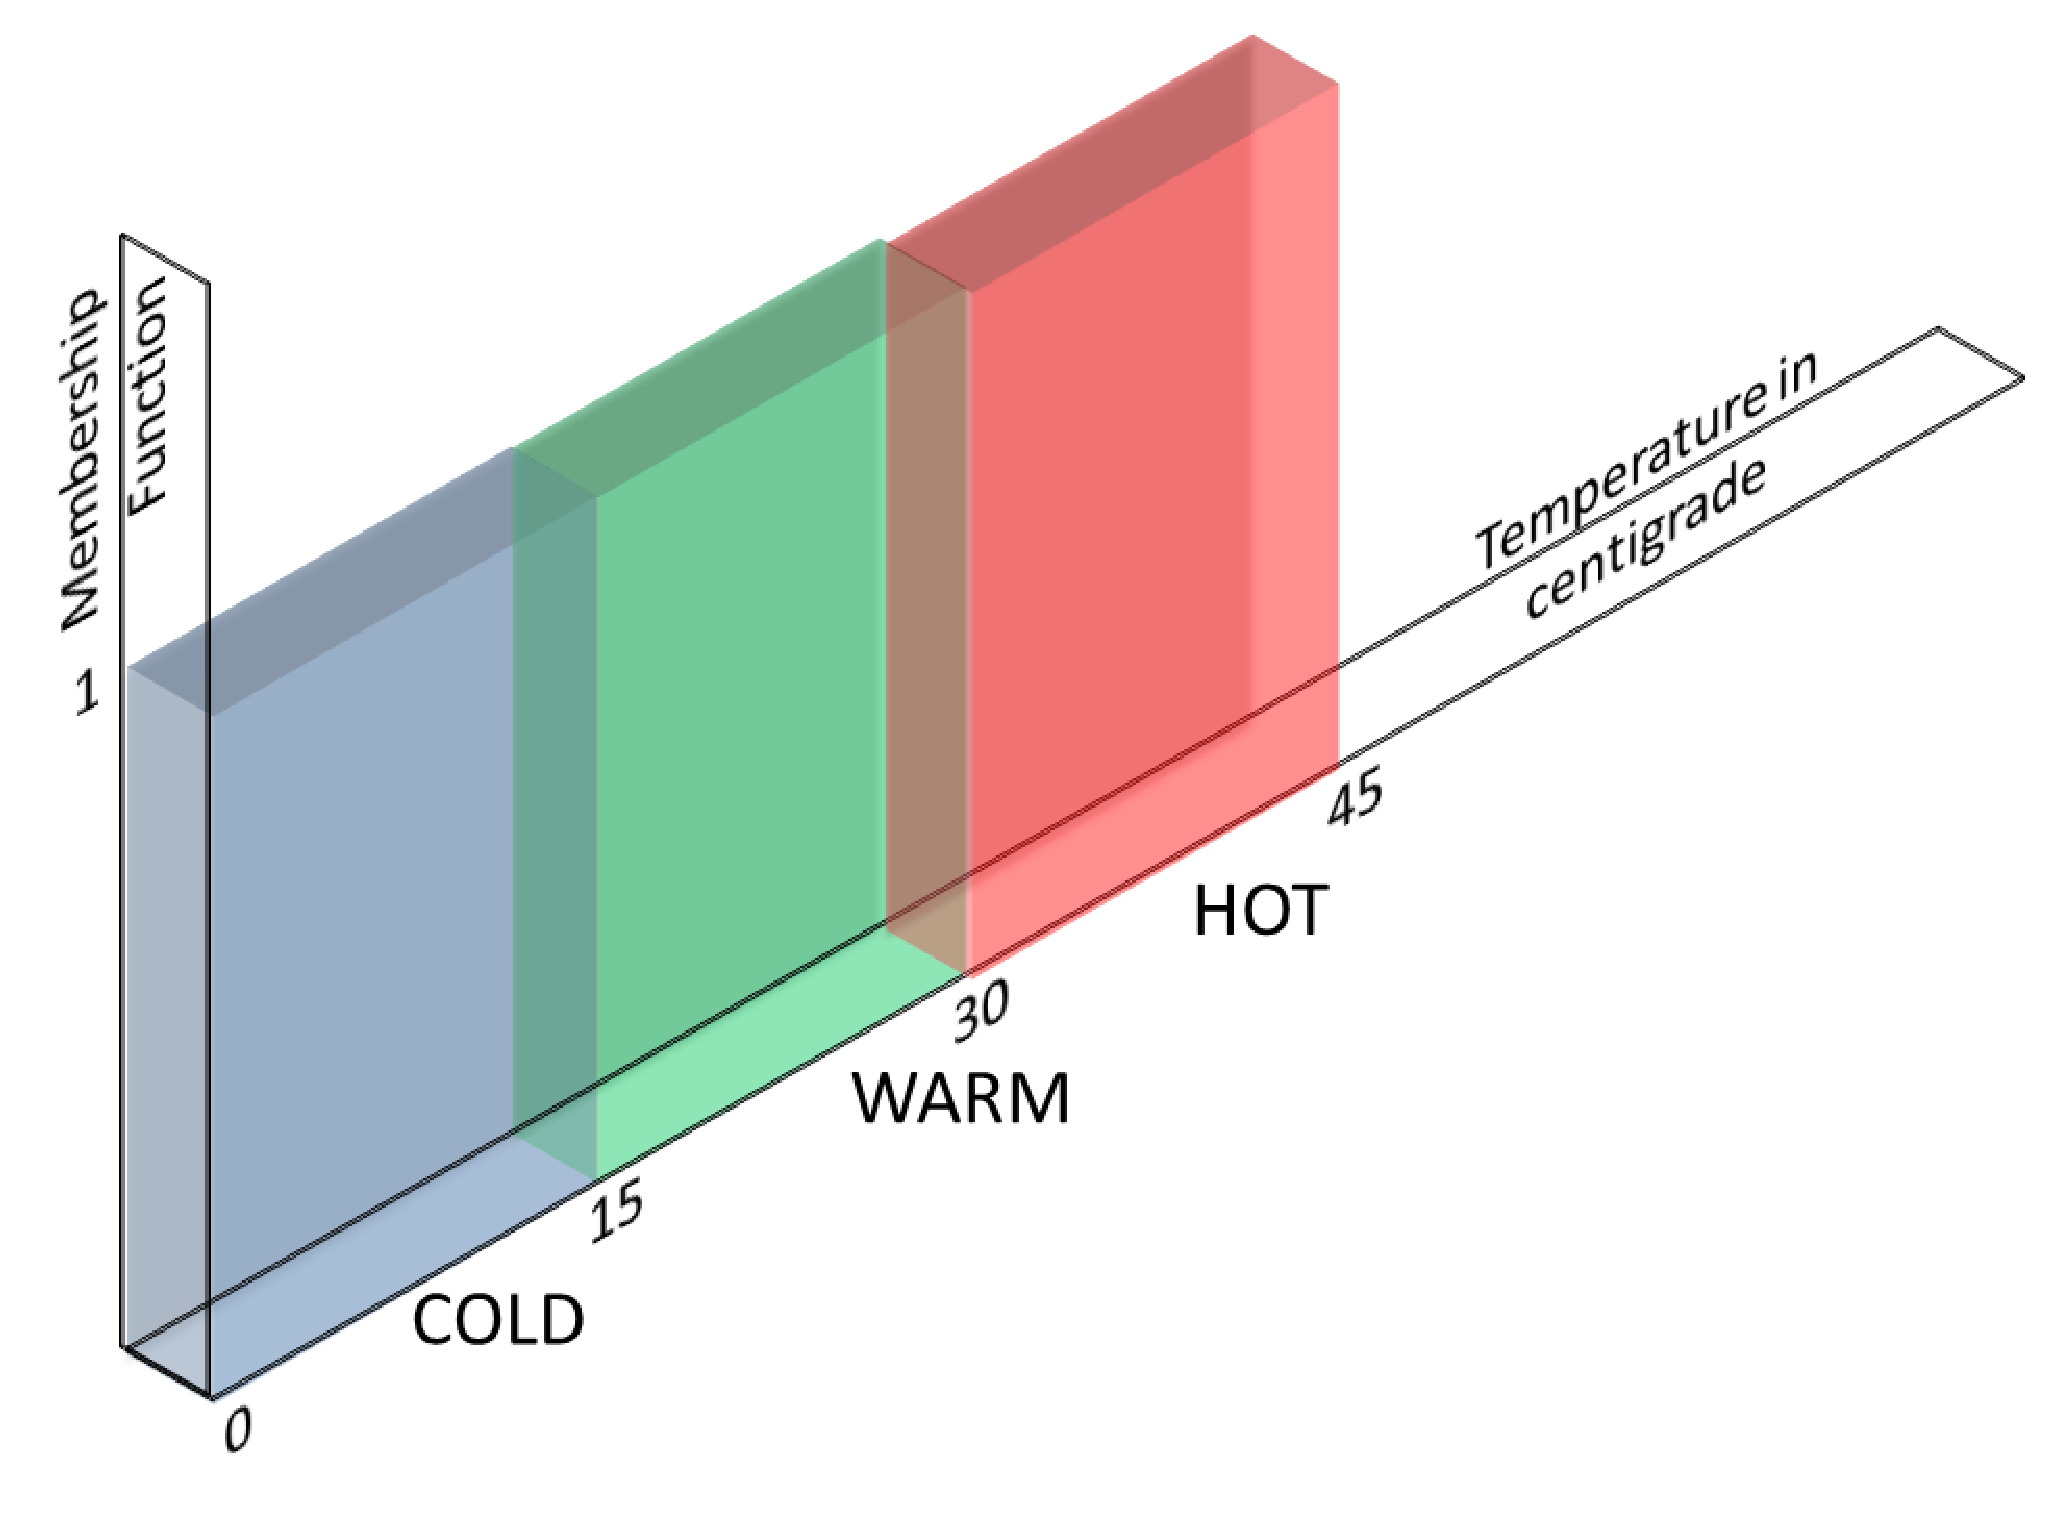
\includegraphics[width=0.8\linewidth]{Chapter1/chapter1/Fig4_b_set}
\caption{Bivalent sets to model room temperature.}
\label{fig:Fig4_b_set}
\end{figure}

 It becomes impossible to generate association  of a variable to more than one set. Based on how human achieves perception, it is inaccurate to model transition from quantity `\textbf{cool}' to `\textbf{warm}' when one degree centigrade of heat is added to the system. The actual modeling in real life however, occurs with a smooth transition or drift from `\textbf{cool}' to `\textbf{warm}'. This transition can be captured if the association itself can be modeled using some functions as depicted in Fig. \ref{fig:Fig5_f_set}. Here, the association is modeled as a triangular function. In fuzzy logic theory, the function which defines the association is called as membership function. Thereby, in fuzzy set theory, apart from the value of the variable, the degree of association of the variable to the set is also captured.
\begin{figure}[h]
\centering
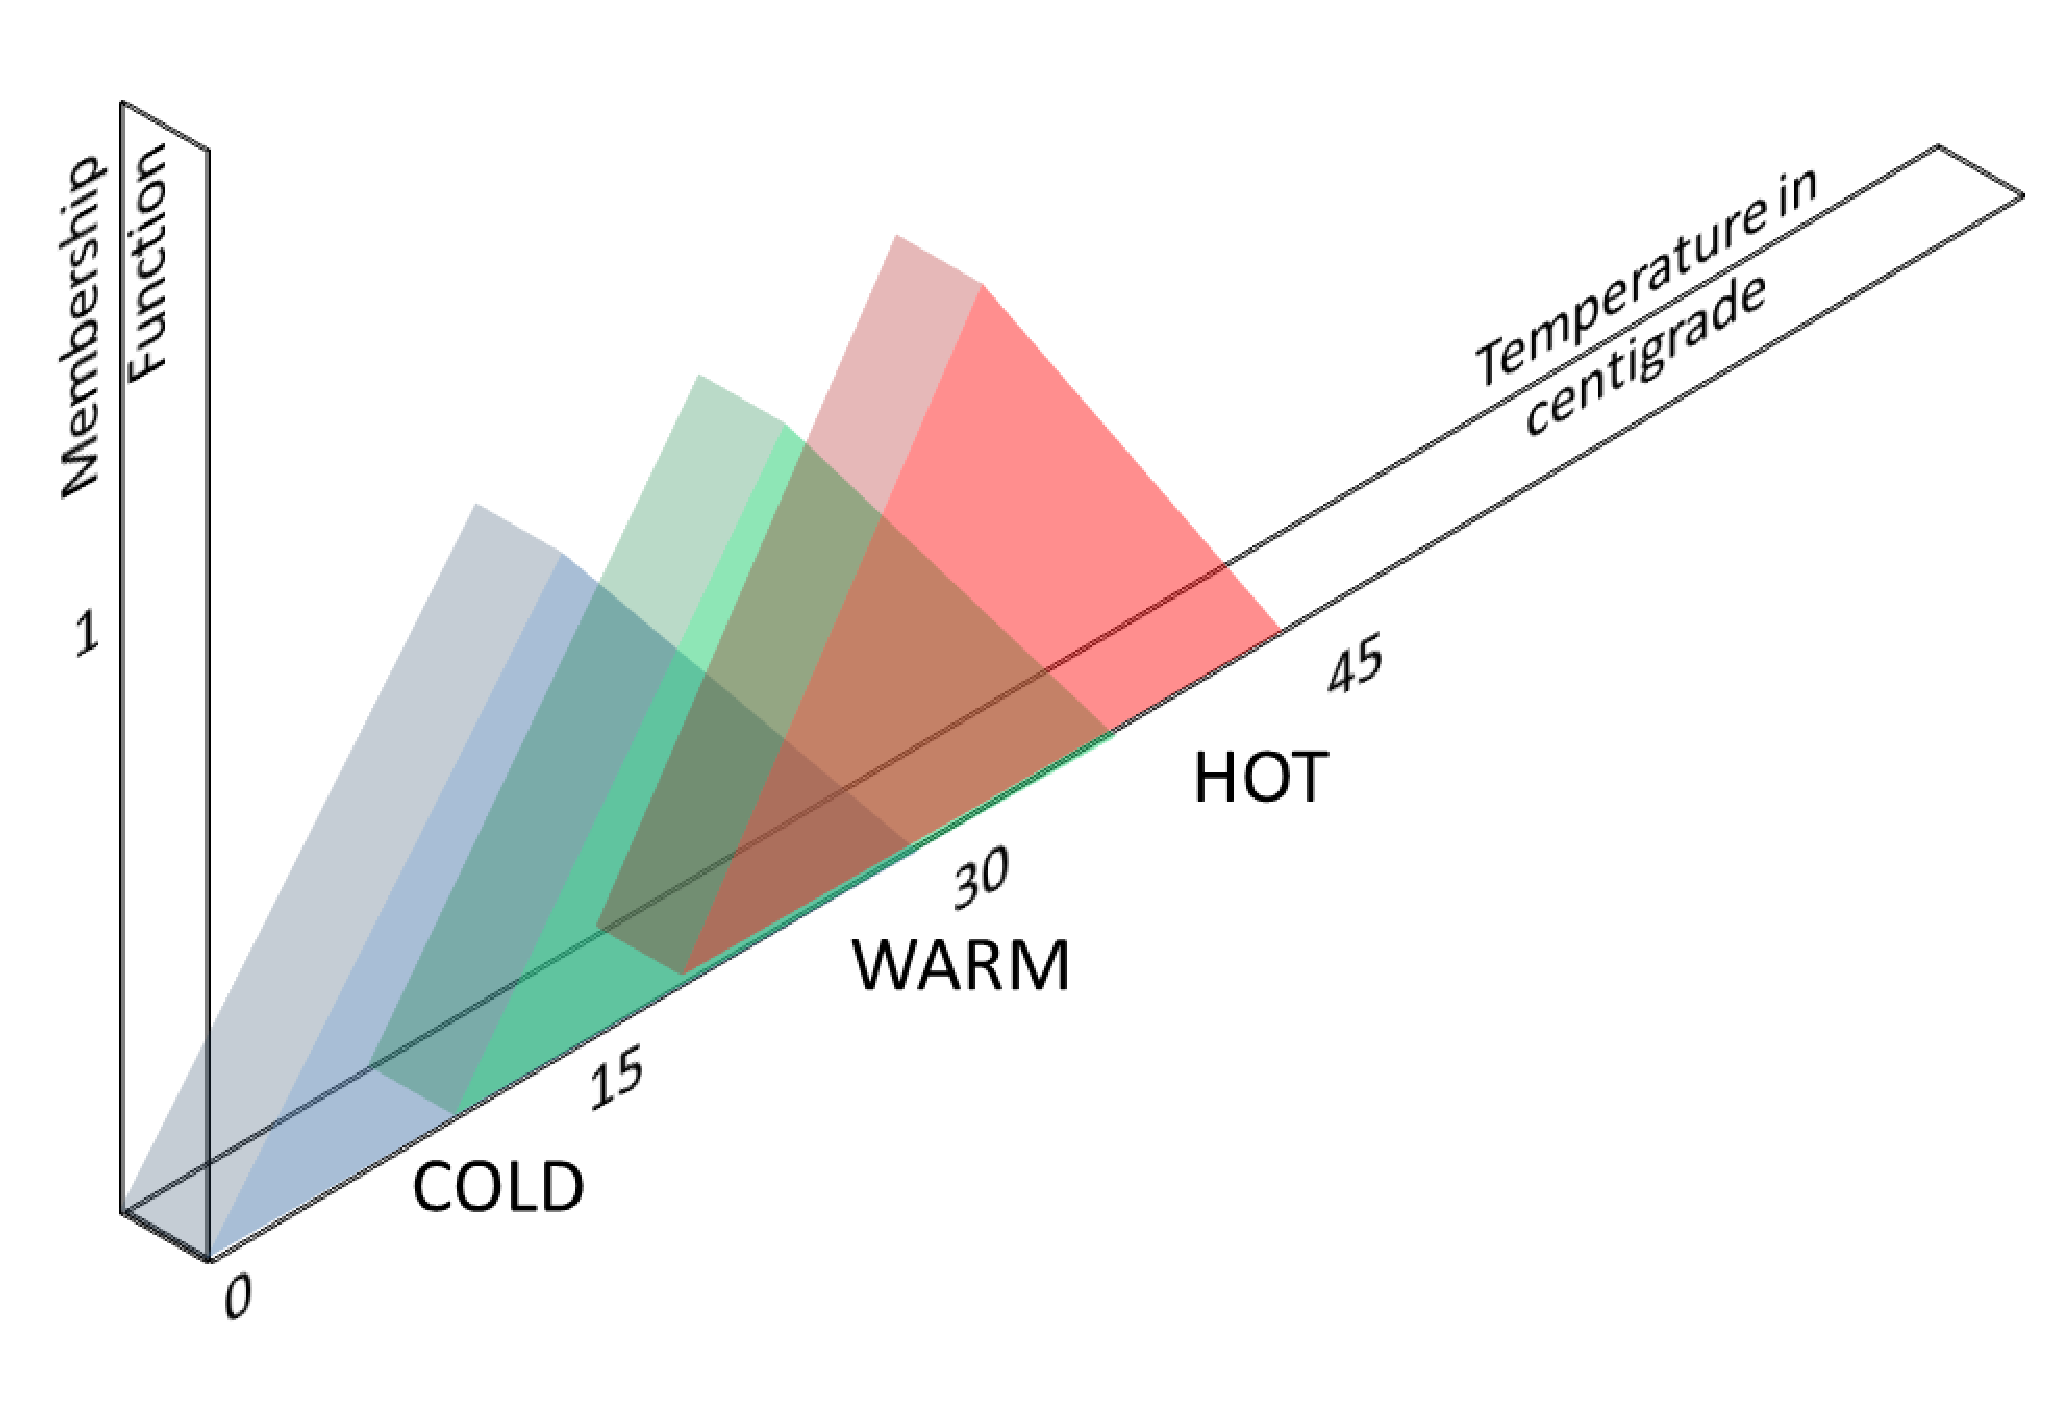
\includegraphics[width=0.8\linewidth]{Chapter1/chapter1/Fig5_f_set}
\caption{Fuzzy sets to model room temperature}
\label{fig:Fig5_f_set}
\end{figure}

Mathematically, a fuzzy set is a pair $ \left( {\xi ,\mu } \right) $, where $ \xi $ is a set, also known as universe of discourse, and $ \mu :\xi  \to \left[ {0,1} \right] $. This implies that $\mu$ presents the degree of association of an element to the set $\xi$ which lies in between $\left[ 0,1\right]  $. Therefore, $ \forall x \in \xi ,\mu \left( x \right) \to [0,1] $, where $ \mu \left( x \right) $ is called the grade of membership for $ x $, $ x $ being a fuzzy number in fuzzy set $\xi$.

A set $\left\{ {x \in \xi |\mu \left( x \right) > 0} \right\}$ is called support and set $\left\{ {x \in \xi |\mu \left( x \right) = 1} \right\}$ is called core or kernel \cite{bookBogdan2006a,Ross2010}. The function $ \mu $ is called membership function (MF) of fuzzy set $ \left( {\xi ,\mu } \right) $\cite{bookBogdan2006a,Ross2010}.

A fuzzy system operates on various fuzzy sets to provide a suitable output. It is often required that these fuzzy sets are combined meaningfully. Various combination operators exist in ordinary set theory, and it is imperative that there exist a commonality of operators between regular and fuzzy sets. These operators are termed as \textit{aggregators} \cite{Nguyen2003}.

\section{Fuzzy Operators}
Ordinary sets are combined or negated by using operators like intersection (AND), union (OR), and complement (NOT) \cite{Nguyen2003}. Similarly in fuzzy sets, minimum, maximum and negation operators approximate AND, OR and NOT operations. However, on many occasion, \textbf{AND} operations can be achieved by functions other than the minimum operation. These functions are collectively referred to as triangular norms or simply as t\hyp{}norms. Similarly, \textbf{OR} operations are referred to as triangular co\hyp{}norms or t\hyp{}conorms or s\hyp{}norms\cite{Ross2010,bookBogdan2006a}.
%bookponce2010,

There are four basic t\hyp{}norms and almost all t\hyp{}norms used in a fuzzy system are derived from these basic operations \cite{bookBogdan2006a}. Consider $\mu _x$ and $\mu _y$ as membership grade of two fuzzy numbers $ x $ and $ y $, in a fuzzy set. Then the following equations represents the various t\hyp{}norm operations in a fuzzy system.
\[\begin{array}{l}
1. \text{Zadeh Intersection:} ~~~T\left( {{\mu _x},{\mu _y}} \right) = \min \left( {{\mu _x},{\mu _y}} \right)\\
2. \text{Product Intersection:} ~~~T\left( {{\mu _x},{\mu _y}} \right) = \left( {{\mu _x} \cdot {\mu _y}} \right)\\
3. \text{Lukasiewicz Intersection:} ~~~T\left( {{\mu _x},{\mu _y}} \right) = \max \left( {0,\left\{ {{\mu _x} + {\mu _y} - 1} \right\}} \right)\\
4. \text{Basic Intersection:} ~~~T\left( {{\mu _x},{\mu _y}} \right) = \left\{ {\begin{array}{*{20}{c}}
	{{\mu _x},~~~if{\mu _y} = 1}\\
	{{\mu _y},~~~if{\mu _x} = 1}\\
	{0,~~~if{\mu _x},{\mu _y} < 1}
	\end{array}} \right.
\end{array}\]

Similarly, the t\hyp{}conorm or s\hyp{}norm operators can be represented as following equations in a fuzzy system \cite{bookBogdan2006a}.
\[\begin{array}{l}
1. \text{Zadeh Union:} ~~~S\left( {{\mu _x},{\mu _y}} \right) = \max \left( {{\mu _x},{\mu _y}} \right)\\
2. \text{Product Union:} ~~~S\left( {{\mu _x},{\mu _y}} \right) = {\mu _x} + {\mu _y} - \left( {{\mu _x} \cdot {\mu _y}} \right)\\
3. \text{Lukasiewicz Union:} ~~~S\left( {{\mu _x},{\mu _y}} \right) = \min \left( {0,\left\{ {{\mu _x} + {\mu _y} - 1} \right\}} \right)
\end{array}\]

There three major fuzzy complement operators which have been widely used in the literature \cite{bookBogdan2006a}. These operators are;
\[\begin{array}{l}
1. \text{Standard Complement:} ~~~N\left( \mu _x \right) = \left( 1 - \mu _x\right)\\
2. \text{Sugeno's Complement:} ~~~{N_s}\left( {{\mu _x}} \right) = \frac{{1 - {\mu _x}}}{{1 + s{\mu _x}}}\\
3. \text{Yager's Complement:} ~~~N\left( \mu _x \right) = \left( {{\mu _x} \cdot {\mu _y}} \right)
\end{array}\] 
where $ s $ is Sugeno's constant and $ w $ is Yager's constant.

\section{Fuzzy Rules}
Words rather than numbers define linguistic variables. Fuzzy rules use these linguistic variables instead of numbers to quantify variables.  These linguistic variables are represented as fuzzy sets with a certain function. This provides the mathematical background of the fuzzy systems. All fuzzy rules are divided into an antecedent part (starting with ``$IF \ldots $'')
and a consequent part (ending with ``$THEN \ldots $''). The antecedent parts describe the causes while the consequent parts describe effects relevant to desired control action. A typical form of a fuzzy rule with Rulebase index $ {R_b}\left( k \right) $ is as shown below.
\[{R_b}\left( k \right):~~~~\text{If}~i_1\text{ is }{a_1}~\text{and}~i_2\text{ is }{a_2}~\text{and}~\cdots \text{and}~i_N\text{ is }{a_N},~\text{then output is }~{c_j}\]
where, $ {i_1},{i_2} \cdots {i_N} $ represents inputs,  $ {a_1},{a_2} \cdots {a_N} $ are called antecedent and $ c_j $ is the resultant consequent.
All antecedents and consequents are represented by valid linguistic variables in a fuzzy system.
\section{Fuzzy Logic Control System}
Traditionally, the industrial process control was dominated by binary logic based reasoning. Heuristic knowledge hardly plays any role in these systems \cite{bookBehera2009,bookMichels2006}. This forced the systems to be represented by a collection of complex mathematical equations. The drive for precise and accurate control was expensive and often proved to respond sluggishly. However, in recent past, the power of human reasoning started to get acknowledged with the advent of FLCS in nonlinear process control \cite{Zadeh1993,Mendel1995,Sugeno1985,Mendel2000}. The most appreciable feature of FLCS is its ability to manage complex control problems through human knowledge and numerical models provided by fuzzy set theory, instead of using complex differential equations to derive mathematical models of  a process plant.

The computing framework of a fuzzy logic control system (FLCS) rely on three conceptual components:
\begin{description}
	\item[i. Rulebase:] This contains a database of rules that represent human knowledge and heuristics. They define I/O relationship of the system in terms of linguistic variables.
	\item[ii. Database:] This defines the MFs that are used to define the linguistic variables in the fuzzy rules. 
	\item[iii. Inference Mechanism:] This performs the reasoning procedure based on the Rulebase and Database.
\end{description}
These three components together constitute the Fuzzy Control Parameters (FCP). At this juncture, an operator's experience and knowledge is appropriately formulated and configured into FCP. This FCP represents the ``intelligence'' in any fuzzy control algorithm. Hence, it can be asserted that the information of the FLCS is dependent on the knowledge of the designer or the operator.

\begin{figure}[t!]
	\centering
	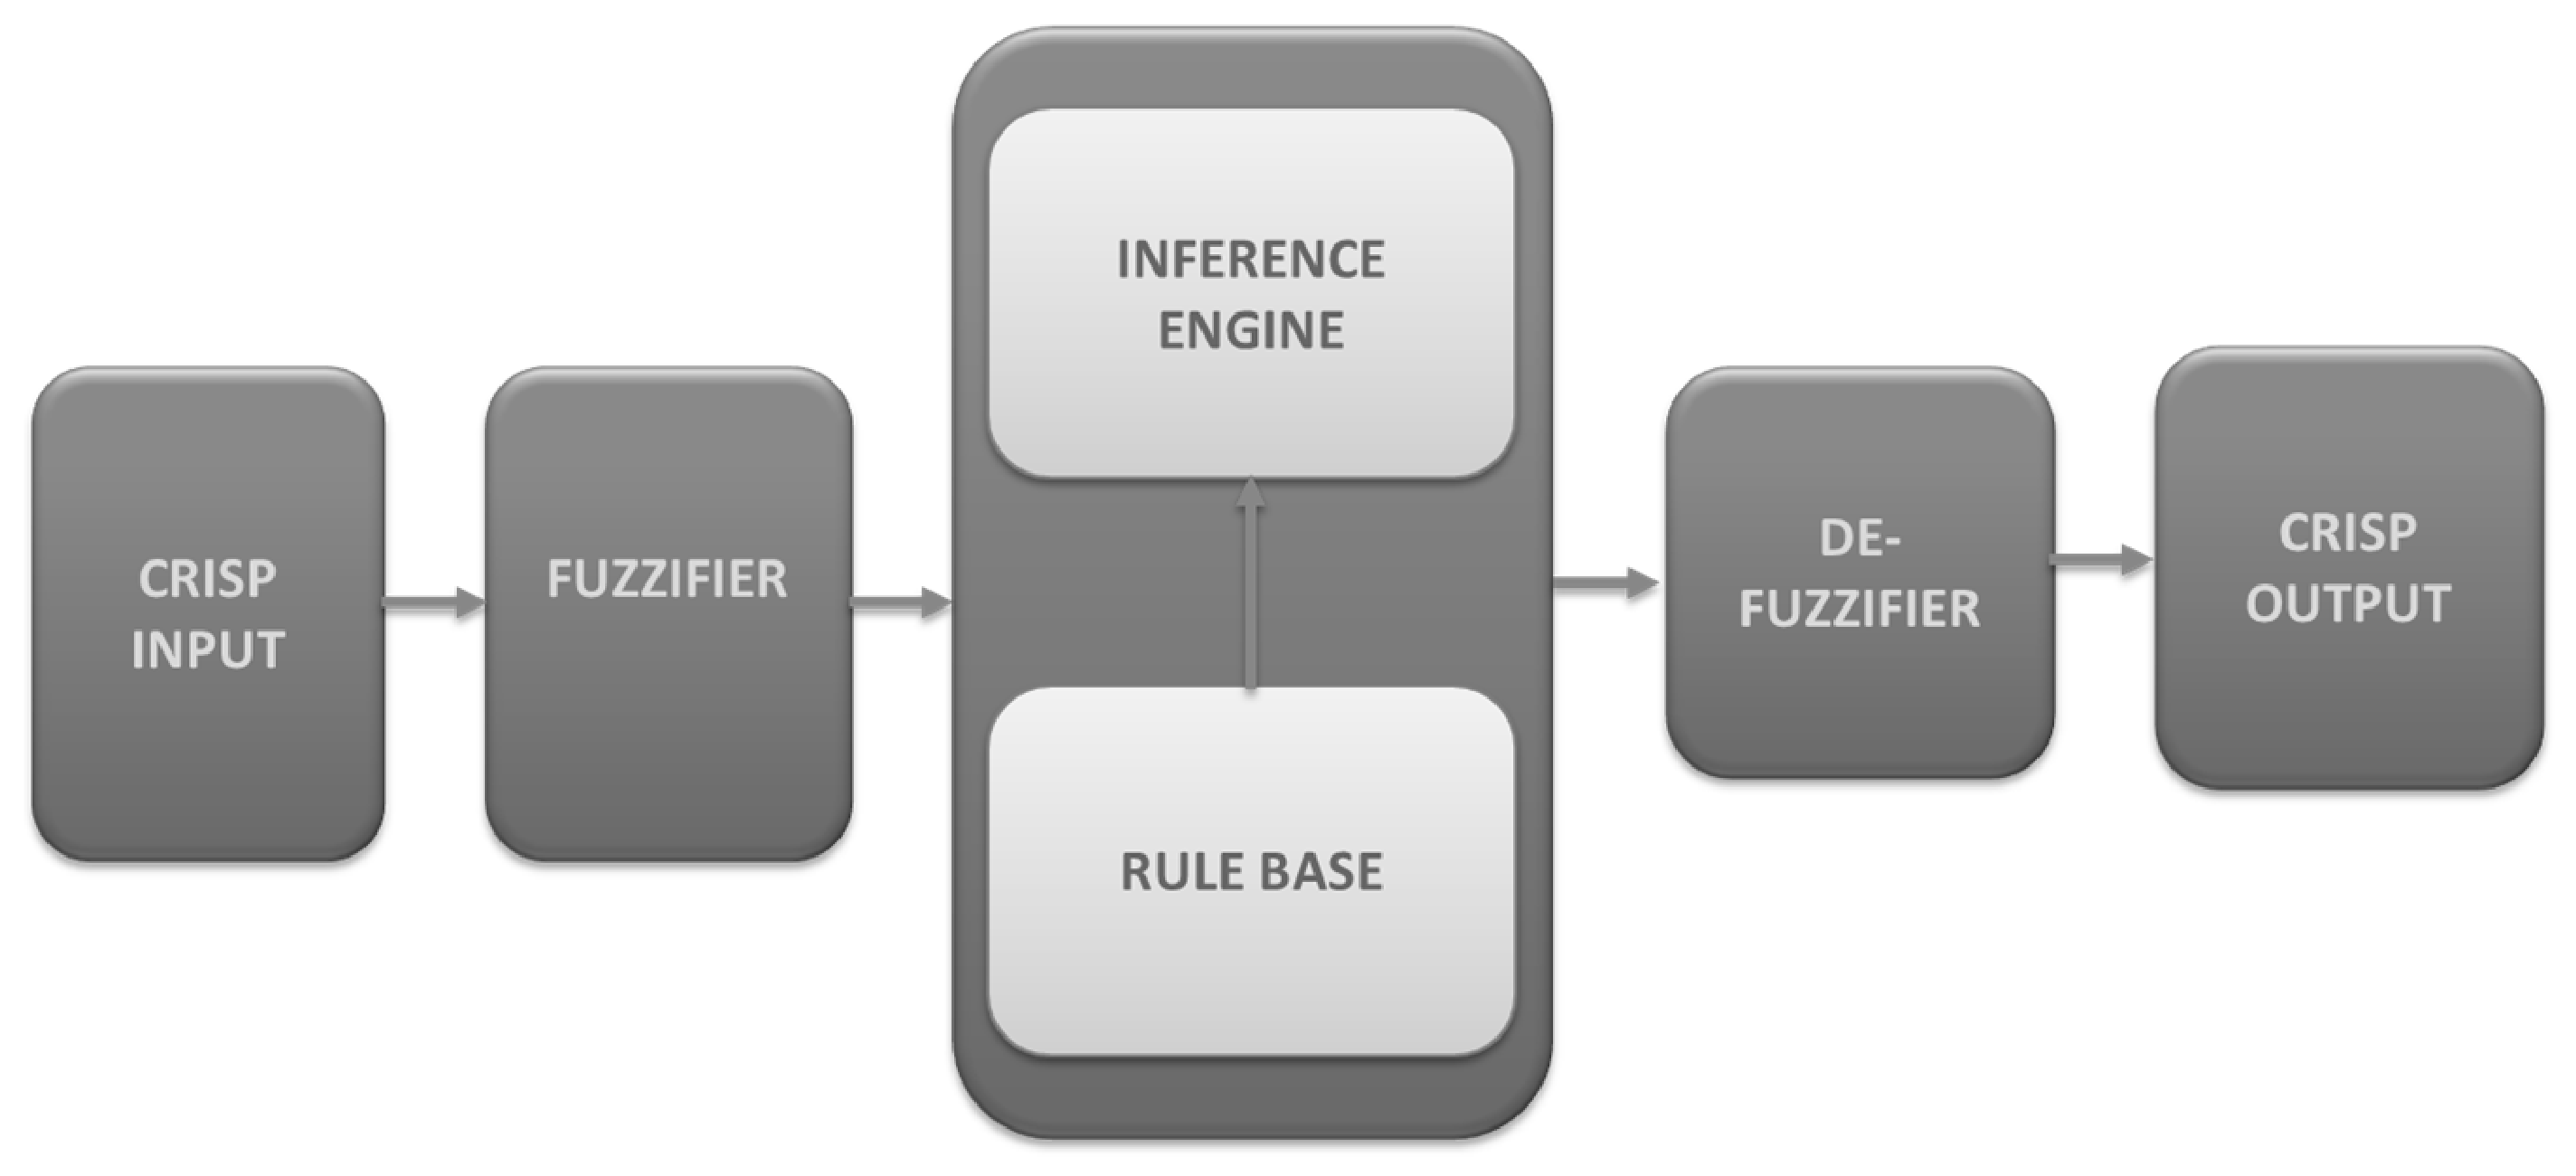
\includegraphics[width=0.9\linewidth]{Chapter1/chapter1/Fig1_FLCS}
	\caption{Black diagram of a FLCS}
	\label{fig:Fig1_1}
\end{figure}

FLCS has four important modules which interact with the input to generate a meaningful output\cite{Wang1997,bookMichels2006,Mendel1995}. The block diagram of the modules in a FLC is represented in Figure \ref{fig:Fig1_1}. These modules are;
\begin{description}
	\item[i. Fuzzifier:] The input variables in a fuzzy control system that are real world variables and also known as \textit{crisp input data}, are in general mapped by sets of membership functions, known as ``fuzzy sets''. The fuzzifier generates a set of output in between 0 to 1, which are dimensionless. This process of converting a crisp input value to a set of fuzzy values is called ``fuzzification''.
	\item[ii. Rulebase:] It stores the heuristic rules that govern a typical fuzzy system. These rules describe the output dependence of the inputs, and they are  mentioned in terms of the MFs representing the inputs and outputs of the process plant.
	\item[iii. Inference Engine] It accepts fuzzified inputs and applies reasoning described by the Rulebase to work out fuzzy outputs.
	\item[iv. Defuzzifier:] It translates fuzzy outputs from the Inference Engine into substantive crisp output applicable to a real system.
\end{description}


\section{Learning of FCP from Data} \label{sec:learnFCP}

Learning of FCP from data essentially means designing or extracting parameters that governs the fuzzy controllers from a given sampled data or model of a system. According to Wang et. al. \cite{Wang1992a} there are five steps in this process. 
\begin{description}
	\item[Step 1] The input and output spaces are recognized and divided into fuzzy regions.
	\item[Step 2] The dataset is observed and fuzzy rules are generated from it.
	\item[Step 3] Each generated rule is assigned a degree to resolve any conflict that arises amongst the generated rules.
	\item[Step 4] Based on visualization paradigm and human expert knowledge, some rules can be directly inferred about the system. These rules are combined with the generated rules.
	\item[Step 5] Once the rulebase is formed, the ouput in fuzzy domain can be obtained. This output is mapped to real world output using a suitable defuzzification procedure. 
\end{description}

In the context of learning FCP, Step 1 to 3 can be manual or it can be formulated as a learning problem itself. G. D. Finn proposed `Fuzzex' for generating fuzzy rules in general from data \cite{finn1999learning}. In this popular technique, they proposed a five step method where cell occupancy is used. But this method does not suit nonlinear system approximation. In 2009, Sánchez et. al., presented a genetic algorithm based learning method which is robust to system noise \cite{sanchez2009genetic}. Tuning fuzzy rules using genetic algorithm has been widely investigated and is often the most popular choice \cite{Surmann2001,Sanz2011,Uddin2007a}. However, learning the entire FCP is a difficult task at hand. To counter this issue, a new strategy for sophisticated learning of FCP with Genetic Algorithm optimization technique is proposed in Section \ref{sec:FCP}. 

\section{Motivation of This work}
PID controllers are widely used in industries even though they are inherently linear and provides a sluggish response. They are generally not suited to control nonlinear process plants \cite{Atherton1999a,Bennett1996,Atherton1999}. Their modeling requires a thorough knowledge of system dynamics and the tuning process is quite difficult too. Fuzzy Logic Controllers (FLC) provide an imprecision based control approach which is fast and reliable. However, they are driven by the human knowledge which is prone to be erroneous. Some designs provide techniques to derive the FCP from a dataset or model. However, this eradicates human knowledge completely. Therefore, it is highly desirable to have a FLCS with two level tuning.
\begin{itemize}
	\item Coarse Tuning: Achieved by using suitable algorithm and FCP are extracted,
	\item Fine Tuning: Using an interface, system is fine tuned by an operator.
\end{itemize} 

\section{Objective of this work} \label{sec:obj}
Fuzzy logic systems have found applications in a variety of fields namely industrial process control, power systems, robotics, water resources, structural design, metallurgy and material science, business and finance, and many more. It is challenging for scientists and engineers to implement an efficient FLCS design that can be integrated into their system of interest, especially if they are not well equipped with knowledge of programming and system development. Therefore, the primary objective of this research is to design and realize a generic fuzzy logic controller system (G\hyp{}FLCS) on a programmable hardware that can be used for a variety of applications without reprogramming. Some of the characteristic features of this proposed control device will include
\begin{itemize}
	\item Plug and play framework: Essentially process plant operators are not good programmers. It is, therefore, mandatory for a controller device to possess a plug and play framework for ease of installation and operation. Users can input the fuzzy parameters through an interactive user interface.
	\item Runtime tunability: Most control device lacks this feature. The major advantage of run\hyp{}time tunability is that it provides an opportunity to include the concept of two level tuning, one of the prime motivating factor for this research. This will offer the leverage to fine-tune the FLCS while it is in operation so that the parameters can be reset to default under critical conditions.
	\item Standalone operation: The prime requirement of any real\hyp{}time system or controller is to be able to operate in a standalone mode.
	\item Flexibility in operation order: A G\hyp{}FLCS system primarily implies that it can be implemented on any system with appropriate parameter tuning; be it a single\hyp{}input\hyp{}single\hyp{}output system or multiple\hyp{}input\hyp{}multiple\hyp{}output system. Thereby, it is implicit that the G\hyp{}FLCS should have the provision to accommodate a different number of inputs and outputs.
\end{itemize}
It becomes a challenging task when run\hyp{}time tunability, flexibility in system order and plug and play framework is combined with the standalone mode of operation. Therefore, the architecture of traditional FLCS is required to be altered in a way such that, the data integrity and operational methodology remains consistent even after incorporating the above-mentioned features.

\section{Literature Survey on Design and Implementations for FLCS on various Hardware Platforms}
%FLC application, need for hardware implementation.
In recent times fuzzy logic is addressing complex problems of control, forecasting and prediction with imprecision in fields of robotics \cite{Linda2011,Acevedo2013,Das2006,Lochan2015,Das2006,Gopinath2008}, chemical \cite{Foerster2013,Pan2005,Aqlan2014,Khoshnevisan2014,Lerkkasemsan2014,Shamiri2015} and manufacturing processes \cite{Zammar2015,Rajak2015,Gokulachandran2015}, automobiles \cite{Wang2015,Baldania2014,Basjaruddin2015,Li2014b,Bogdan2008}, business and finance\cite{Korol2014,Tung2004,Yoshida2003,Dostal2013}, power electronics \cite{Bhende2006,Lou2015,AlNabulsi2012}, and many others\cite{Dostal2013,Kumar2015,Kumar2015a,Sun2015,Boumaaraf2015,Jadoun2015} in a better way than conventional control techniques. Wide spread application of the FLCS and its extensively high effectiveness to a larger extend
is driven by formalizing necessary human knowledge and sometimes behavior in the controller as an imprecise and approximate representation. These factors impel engineers to design and implement fuzzy based controllers for wide array of applications.

The hardware designs of FLCS can be classified into three broad categories based on their circuit architecture.
\begin{itemize}
	\item Analog, 
	\item Digital, and  
	\item Mixed Signal
\end{itemize}
Each of these can be further classified based on the aspect of system design and platform for implementation. 
\begin{description}
	\item[Dedicated Integrated Circuits:] These FLCS are designed primarily to target a single control application. These devices are mostly built over application specific integrated circuits (ASIC) and implement full custom analog, digital or mixed-signal designs \cite{Idros2014,Matsumoto2014,Li1997,Gomariz1998,Malek2008,Costa1995}.
	\item[Programmable Integrated Circuits:] Programmable Integrated Circuit based FLCS devices are commercially developed in integrated circuits (ICs) that can be reconfigured by the user. These tools provide attractive options to designers and engineers. They have the ability to be reprogrammed, and their high integration density is a fascinating feature. Commercially available field programmable gate arrays (FPGAs) and field programmable analog arrays (FPAAs\footnote{This is an integrated device comprising of configurable analog blocks (CAB) and in between interconnects. Lattice and Anadigm are prime manufacturers of this device.}) have been widely used in designing of these systems \cite{Guajardo2007,Sun2015a,Monmasson2007,Cecati2010,Palakeerthi2014,Jabeen2008,Tran2015,Pierzchala1998}.
	\item[Commercial Processors:] A software application defining the system is developed and deployed on these devices. Microprocessors ($\mu$P), Microcontrollers ($\mu$C) and Digital Signal Processors (DSPs) based systems are defined under this category \cite{Santoso2014,Youness2014a,Kurniawan2015,Yousef2015,Jia2011,Oswald2014,Selvaperumal2014}.
\end{description}

\begin{table}[t!]
	\centering
	\caption{Taxonomy for Hardware Implementation of FLCS}
	\label{tab:tax}
	\begin{tabular}{clll}
		\hline
		\multicolumn{1}{l}{} & Classification & Platform & Devices \\ \hline
		\multicolumn{1}{c|}{\multirow{9}{*}{\begin{tabular}[c]{@{}c@{}}Types of\\ Implementation\end{tabular}}} & \multicolumn{1}{l|}{\multirow{3}{*}{Analog}} & Dedicated IC & Analog ASIC \\
		\multicolumn{1}{c|}{} & \multicolumn{1}{l|}{} & Programmable IC & FPAA \\
		\multicolumn{1}{c|}{} & \multicolumn{1}{l|}{} & Commercial Processor & -- \\ \cline{2-4} 
		\multicolumn{1}{c|}{} & \multicolumn{1}{l|}{\multirow{3}{*}{Digital}} & Dedicated IC & Digital ASIC \\
		\multicolumn{1}{c|}{} & \multicolumn{1}{l|}{} & Programmable IC & FPGA, CPLD \\
		\multicolumn{1}{c|}{} & \multicolumn{1}{l|}{} & Commercial Processor &  \\ \cline{2-4} 
		\multicolumn{1}{c|}{} & \multicolumn{1}{l|}{\multirow{3}{*}{Mixed}} & Dedicated IC & Mixed Signal ASIC \\
		\multicolumn{1}{c|}{} & \multicolumn{1}{l|}{} & Programmable IC & -- \\
		\multicolumn{1}{c|}{} & \multicolumn{1}{l|}{} & Commercial Processor & -- \\ \hline
	\end{tabular}
\end{table}

Different forms of FLCS implementation is presented in Table \ref{tab:tax}. The forms of FLCS include;
\subsection{Analog Implementation of FLCS Design}
A Large number of FLCS in literature have been developed on analog devices. The major reasons that drive a FLCS design engineer to choose these platforms are high parallelism, high speed, low area and low power consumption \cite{Soleimani2010,Soleimani2014,Baturone1996,Peyravi2002}. Different forms of Analog IC based implementation includes;
\subsubsection{Dedicated IC based FLCS}
There are three modes in which these devices are implemented namely,
\begin{description}
	\item[Current Mode] implementation uses fewer transistor and hence they consume low power. However, these devices can only connect to one output since they work in current mirror mode \cite{Bosque2014b,Zavala2012}. Some of the work those were developed using these techniques are
	\begin{itemize}
		\item Tokmakci et. al.\cite{TokmakcI2008} designed current\hyp{}mode CMOS FLC. The membership function circuit (MFC) implemented trapezoidal, triangle, Z\hyp{}shape and S\hyp{}shape MFs. which were tunable by two voltages through switches.{ The system developed was a two\hyp{}inputs\hyp{}one\hyp{}output with 9 tunable rules only}. The operation speed of this FLCS was reported to be 6.25 Mega Fuzzy Logic Inferences per second (MFLIPS)\cite{TokmakcI2008}.
		\item Gheysari et. al.\cite{Gheysari2011} proposed a Flexible Structured Fuzzy Logic Controller Chip (FS\hyp{}FLC) on $ 0.35 \mu m $ process. They implemented Ordered Weighted Averaging operator to aggregate multiple\hyp{}input single\hyp{}output (MISO) system.{ However, the FLCS design used singleton rules at output. }
	\end{itemize} 
	\item[Voltage Mode] implementation of FLCS can serve more than one outputs unlike current-mode. Some of the noted designs include
	\begin{itemize}
		\item Mokarram et. al.\cite{Mokarram2015}: developed a two\hyp{}input, single\hyp{}output Takagi\hyp{}Sugeno\hyp{}Kang (TSK) FLC on $ 0.35 \mu m $ standard CMOS process. The system supports triangular and trapezoidal membership functions. Membership function generator (MFG) provides generation and tuning of the MFs but {the design do not permit changing or tuning of rules}.
		\item Aminifar et. al.\cite{Aminifar2012}: The designed a FLCS on $ 0.35 \mu m $ CMOS process with inference speed of 14.83 MFLIPS. {They designed a 2\hyp{}input one\hyp{}output system with mere 9 rules with support to only singleton MFs at output. Moreover, the design do not allow any tunability.}
	\end{itemize} 
\end{description} 

\subsubsection{Programmable IC based FLCS}
There has been very limited research reported on FLCS implementationAnalog Programmable ICs. Some of the most significant works include;
\begin{itemize}
	\item Amaral et. al\cite{Amaral2004} designs and developed in PAMA\hyp{}NG, a FPAA platform, with I/O board connected to the PCI bus of the PC. The system used Genetic Algorithm (GA) to reconfigure the FPAAs. 
	\item Ionita et al.\cite{Ionita2005} also used evolutionary algorithm to tune MFs. They developed a Mamdani type FLCS on FPAAs.
\end{itemize}
{It has been observed that designs implemented on Analog Programmable ICs are extremely sensitive to problems of fanout and presence of switches on the signal path \cite{pierzchala2013field}. It is also known that analog circuits are more vulnerable to be affected by noise in comparison to Digital circuits.}

\subsection{Digital Implementation of FLCS Design} 
Fuzzy systems and control are making fast advancement in past decade and two. Owing to its pragmatic achievements in consumer electronics and industrial process control, implementation of FLCS has been rigorously researched and developed. However, increase in process complexity of the industrial plants is accelerating demand for controllers with high computational speed, low complexity, easy deployment, comfortable handling and less development time in terms of design. {In order to conform to the demand\hyp{}supply chain of the industry, FLCS have to be designed accordingly.} A noteworthy solution to fulfill this growing market demand is to move to a digital platform. It is well known that digital systems have high resistance to noise, temperature and voltage variations. There is a vast array of digital platforms available to an engineer for design implementation that reduce turnaround time. Although, systems designed in digital hardware platforms are not as fast as analog designs; still a good system cycle time can be achieved which provide sufficient throughput speed for the majority of the control problems. Table \ref{tab:tax} shows the various digital implementation platforms for realization of different FLCS designs.

\subsubsection{Dedicated IC based FLCS}
These implementations concentrate on structuring the fuzzy rules in a FLCS and its functionality is defined by, whether these rules are evaluate sequentially or in parallel. Some of the notable designs include
\begin{itemize}
	\item Eichfeld et. al.\cite{Eichfeld1992} reported a four\hyp{}input single\hyp{}output FLCS with 4096 rules with eight MFs for each input. However, the system {operated only on two overlapping MFs and used singleton type MFs for output}.
	\item Jacomet et. al.\cite{Jacomet1996} described an architecture of a VLSI fuzzy processor fabricated in the $ 0.7 \mu m $ digital CMOS process. High performance was achieved due to its parallel architecture. The FLCS evaluates 64 rules but {this design too uses two overlapping MFs scheme. Moreover, if four inputs are used, the rules are limited to 64 and thereby, only 3 MFs per input were allowed}.
	\item Huang et. al.\cite{Huang2005} developed a FLCS in $ 0.35 \mu m $ CMOS process. {However, this design used trapezoidal MFs only with a fixed rulebase.}
	\item Hamzeh et. al.\cite{Hamzeh2009} designed one of the most flexible structure for FLCS in the literature. {This device however do not discuss the speed of performance.}
	\item Javadi et. al.\cite{HajiSeyedJavadi2012}'s design provides a new fuzzification method for hardware on $ 0.13 \mu m $ but it is {only applicable to piece\hyp{}wise linear MFs.}
\end{itemize}

\subsubsection{Programmable IC based FLCS}
\paragraph{CPLD based FLCS Design}
It has been shown in Table \ref{tab:tax} that there are two preferred devices which can be categorized in this segment, namely FPGA and complex programmable logic device (CPLD). There are very few CPLD based designs reported in literature. Some of the important designs are,
\begin{itemize}
	\item Hongguo Sun et. al. \cite{Sun2013} presented a Fuzzy PID design on CPLD for PWM trigger pulse generation to a full bridge inverter and a chopper circuit. {It implemented a two\hyp{}input one\hyp{}output FLCS with fixed rulebase and rigid MFs}.
	\item Jingyan Xue et. al. \cite{Xue2009} presented a novel methodology to design a fuzzy reasoning based expert system on CPLD for fault diagnosis. Similar to previous design,{ this too implemented a FLCS with fixed rulebase and rigid MFs.} 
\end{itemize}
There are not many CPLD based FLCS designs that are reported in literature. The decisive reasons are that CPLDs are cost and power intensive platform. Moreover, there are platforms which are easy to configure than CPLDs.

%INCLUDE FPGA based LIT SURVEY
\paragraph{FPGA based FLCS Design}

\begin{itemize}
	\item Adhavan et. al. \cite{Adhavan2014a} countered the problem of non-uniform variance of the torque developed in a vector controlled permanent magnet synchronous motor by introducing a FIS implemented on an FPGA. Author have reported that the heuristic knowledge based FLCS (Fuzzy Logic Control System) has reduced the torque ripple to 1.81\%.
	\item Ben, Zekeri et al. \cite{Benzekri20146109} reported PD approximated FLCS developed on cyclone II FPGA to control a dual axis sum tracking systems.  The simple rules developed with human knowledge have been found to be successful in reducing chip count, cost and development time of the controller significantly.
	\item Santo and Ferreira \cite{Santos2014} implemented a multi-state FLCS on virtex II FPGA and NI compact $ R10-9002 $ to control servo- pneumatic actuation systems.  They showed significant performance gain in term of steady state error, overshoot and settling time.
	\item Messai et. al. \cite{Messai2011} reported a FLC to seek maximum power point deliverable by a photovoltaic (pr) module using measures of PV voltage and current.
	\item Schriber et. al. \cite{Schrieber2015}presented an interval type- II FLCS implemented on a xiling spartan 6 FPGA utilizing DSP48AI slices for different linear and non-linear modules.
	\item Tamukoh et. al. \cite{Tamukoh2007} reported a new technique of bit shift based fuzzy inference method for an efficient digital hardware implemented. They implemented the proposed design on a virtex II FPGA for a self-organization relationship network. 
\end{itemize}
	These designs depicts that the realization of FLCS on FPGA development platform is fast and efficient. However most of these designs are application specific. It is important to realize that even  the speed achieved by these designs cannot to achieved by any generic FLCS design as these appears a large amount of branching in the G-FLCS algorithm.	
\paragraph{Digital ASIC Design based FLCS Design}	
	\begin{itemize}
		\item Martinez-rodriguez \cite{Martinez-Rodriguez2015} has presented a FLCS on ASIC platform where the number of input to and output MFs can be varied on run time. {However, in this design, the number of configurable parameters are very few with a rigid rulebase.}
		\item Evmorfopoulos et. al. \cite{Evmorfopoulos2002} reported a G\hyp{}FLCS structure on digital ASIC which can {had a maximum of five MFs at the input. All input MFs were Gaussian type and output MFS are singleton type.}
		\item D'Amore \cite{DAmore2001} reported a bit scalable fuzzy processors with three input and MF generators. {However like the previous design, this system do not equate with output MFs other than singleton type too. }
	\end{itemize}
	Digital ASIC design is generally quite time intensive in development and the process incurs extreme cost. Without large production, these designs are not cost-effective solution.
%INCLUDE DSP based LIT SURVEY
\subsubsection{Commercial Processors based FLCS}

\paragraph{FLCS Implementation with TMS320F Series DSP}
\begin{itemize}
	\item EL Khatib et. al. \cite{ElKhateb2014} presented a FLCS based SEPIC converter on TMS32F28335 DSP device to successfully track the reference signal using MPPT to transfer power around 4.8\% than conventional PI based system.
	\item Eskandarin et.al \cite{Eskandarian2014} proposed a fuzzy instantaneous power theory to improve conventional p-q theory dynamic performance and implemented it on a TMS320F28335 DSP device.
	\item Okumus et. al. \cite{Okumus2014} has reported on FLCS design implementation of TMS320F2812 DSP device to control a brushless DC motor and compared the result with HB current controller. The heuristic knowledge based FLCS is found to perform extensively well.  
\end{itemize}

\paragraph{FLCS Implementation with TMS320C Series DSP}
\begin{itemize}
	\item Uddin et. al. \cite{Uddin2007} showed a cost effective FLCS based controller designs on TMS320C31 DSP to control an interior permanent magnet synchronous motor for high performance industrial applications.
	\item S. Gai et al. \cite{Gai2010} used a TMS320C6713 DSP device to implement a fuzzy based Haar wavelet feature extraction technique to successfully classify and detect a counterfeit banknote.
\end{itemize}

\paragraph{FLCS Implementation with dSpace DSP}
\begin{itemize}
	\item Butt et. al. \cite{Butt2004} implemented FLCS based MTPA speed control of a IPMSM drive on a DS1102 DSP.
	\item Like many FLCS designs reported on tracking of maximum power point using MPPT algorithm Noman et. al. \cite{Noman2013} also proposed a FLCS design for similar application using a DS1104 DSP.
	\item Rafa et. al. \cite{Rafa2014} implemented a new FLCS design on DS1104 DSP to solve coupling problem in vector control of induction motor.
	\item Rubaai et. al. \cite{Rubaai2007} used DS1104 to implement a FLCS control structure with adaptive la based Lyapunov synthesis for trajectory tracking control of a brushless servo drive systems.
\end{itemize}

There are many more DSP based FLCS designs that have been successfully implemented in various control applications. It can be readily inferred that the development of DSP based FLCS is easy compared to FPGA \cite{Parker2010,Lall2002Xilinx,Schneiderman2014}. However, since the parallel architecture can be implemented on FPGA, DSP likes sequential processors are preferred less while developing application specific FLCS \cite{altera2007}. Moreover, the number of branching infractions are extensively reduced in application specific FLCS design as the fuzzy parameters are fixed. This makes FPGA platform more preferable. However for GFLCS design, the situation is quite inverse. In next section, it will be explained why DSP is preferred over FPGA for this particular research work.

\section{Inference from the Literature Survey}
The previous section have laid down the various FLCS designs and some essential features in their implementation. It would be beneficial to summarize the prime aspects of these designs. In this section, a brief inference of the literature survey is portrayed.
\subsection{FLCS Implementation in FPGA and DSP Platforms}
FPGAs and DSPs are most widely used programmable devices for digital implementations of various algorithms \cite{Jinghong2007,Buccella2012,Bilsby1998}. Traditionally, manufacturers like Texas Instruments(TI) and Analog Devices developed processors for specifically for signal processing applications and called them DSP. These are most still most preferred platform for signal processing applications \cite{Lall2002Xilinx}. However, the unsatisfiable need for gadgets that require higher performance and address complex algorithms is driving growth that is hard to keep up with. FPGAs have emerged as a solution to the much needed reconfigurable platform and are capable of addressing the design challenges of large and complex algorithms. However, algorithms that do not confront very high algorithmic complexities are still realized in DSPs \cite{Lall2002Xilinx,Adams2002wp}. TI reported that car manufacturers like BMW, Audi, and Toyota were using DSPs for driver\hyp{}less cars. DSPs have also been reported to manage the real-time processing of visual data for advanced driver assistance systems (ADAS) applications in the main automotive products \cite{Schneiderman2014}.

Many researchers have implemented FLCS on FPGA and DSP platforms. Figure \ref{fig:Fig2_FPGA} and Figure \ref{fig:Fig3_DSP} clearly shows that these are two of the most preferred platform for FLCS implementation.

\begin{figure}[t!]
	\centering
	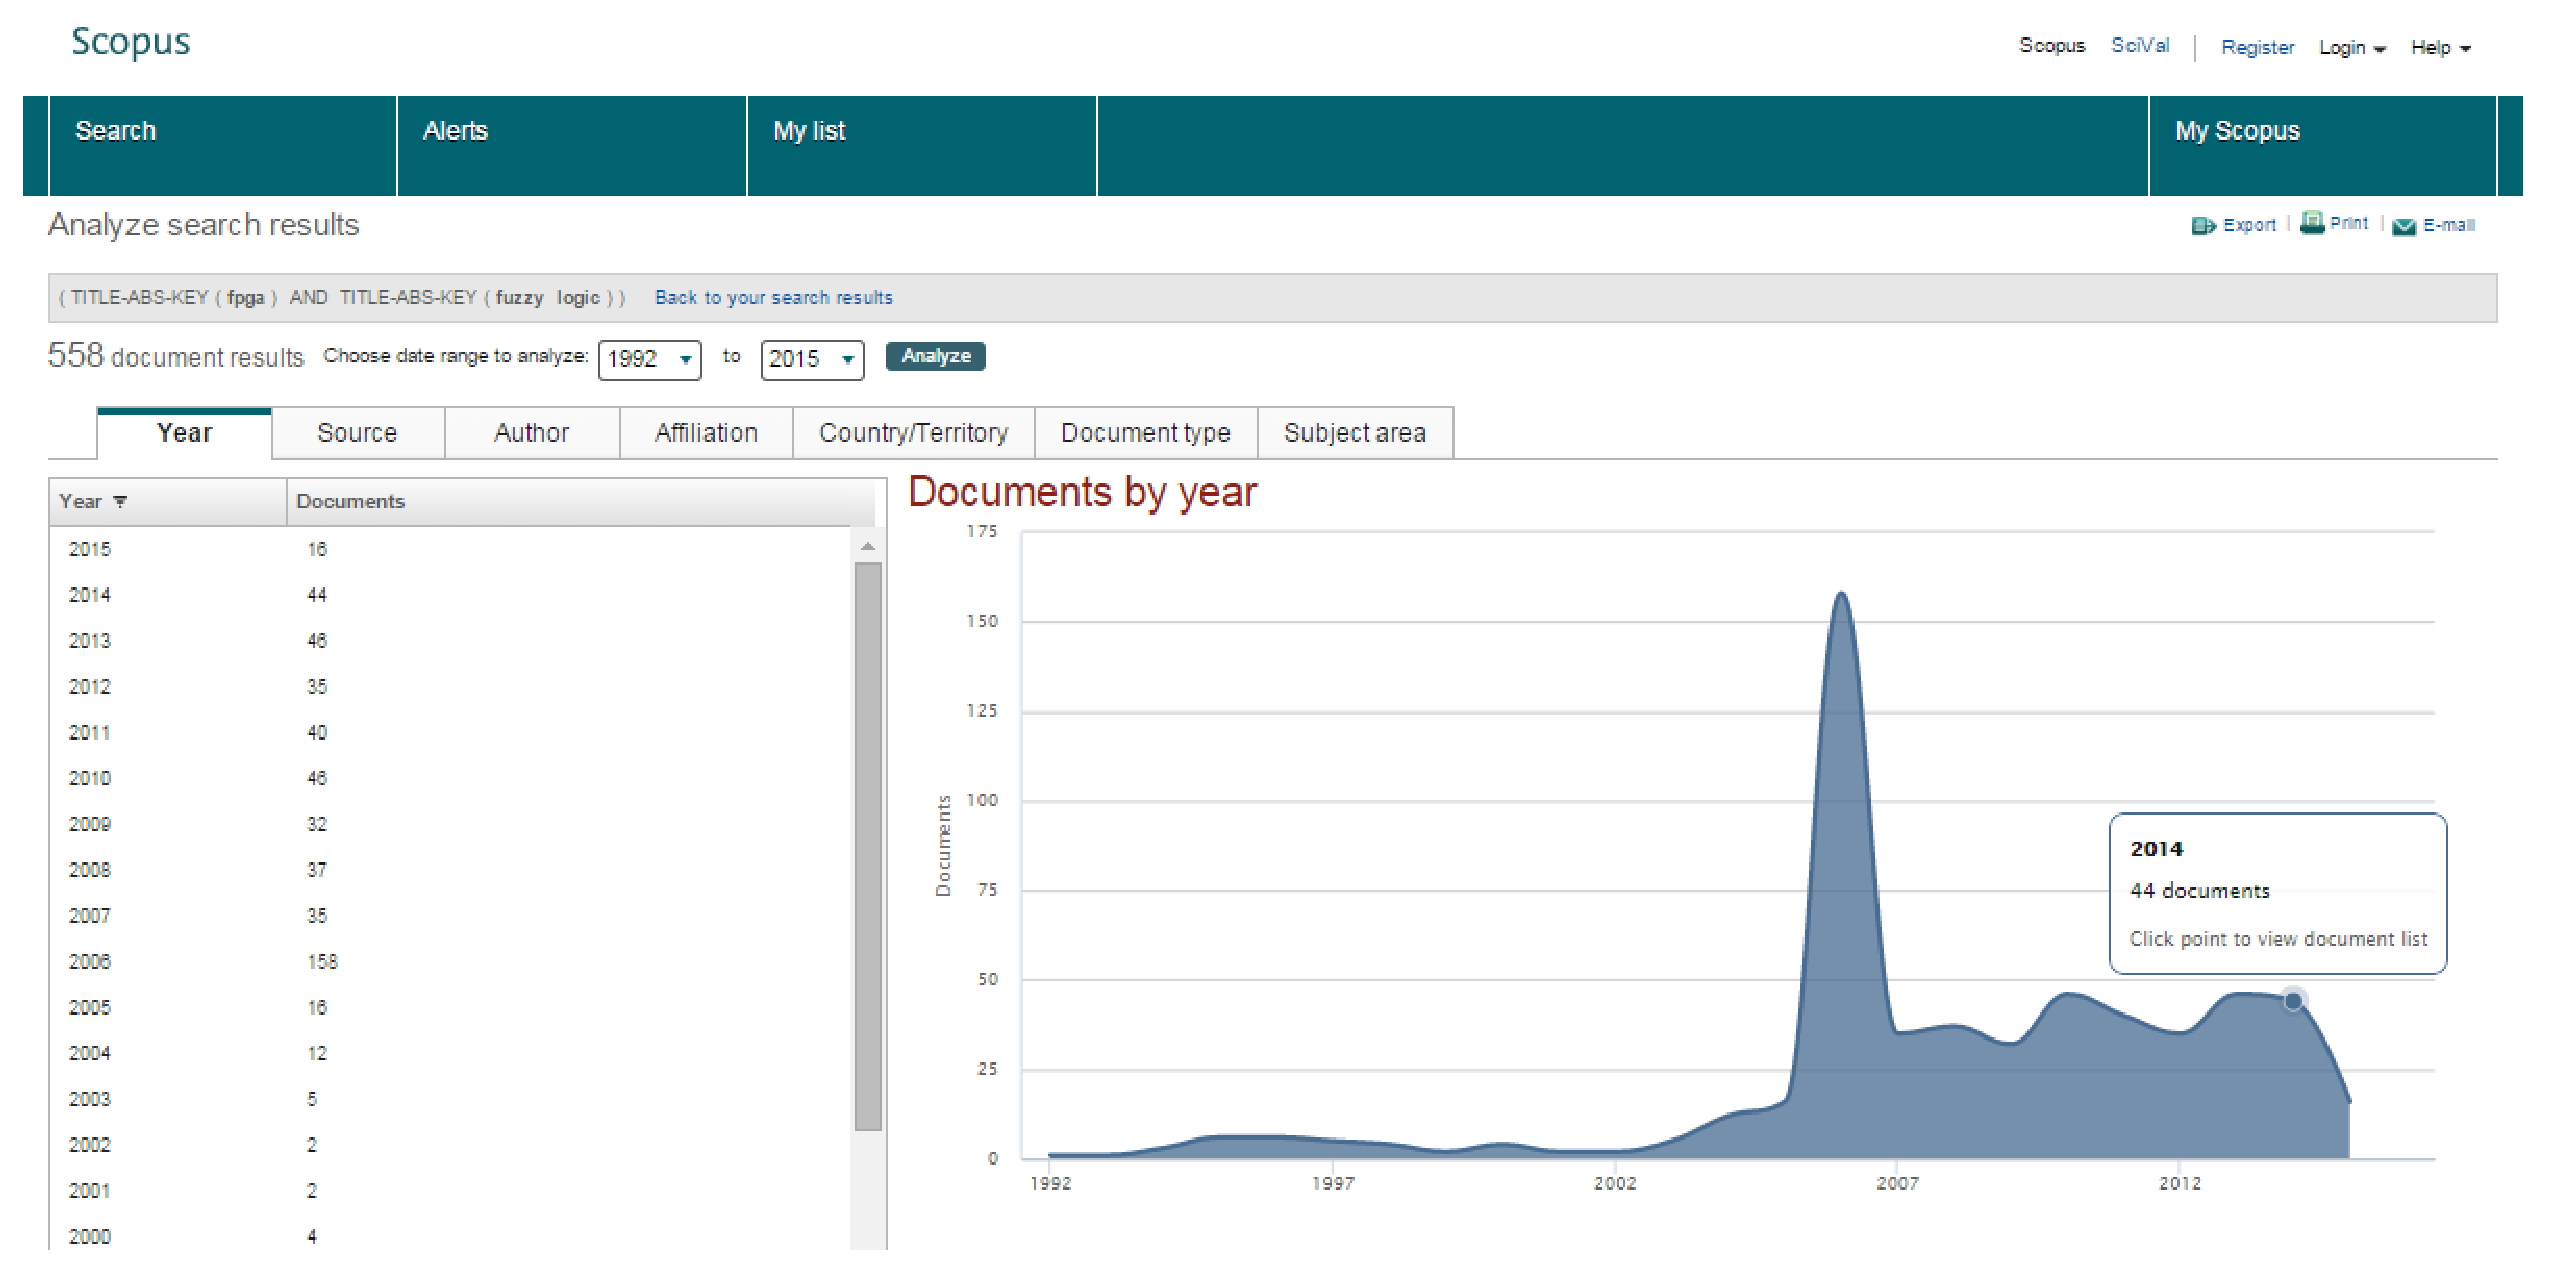
\includegraphics[width=1\linewidth]{Chapter1/chapter1/Fig2_FPGA_trend}
	\caption{Literature on FPGA implementation of FLCS as reported by scopus as on May 2015}
	\label{fig:Fig2_FPGA}
\end{figure}
\begin{figure}[t!]
	\centering
	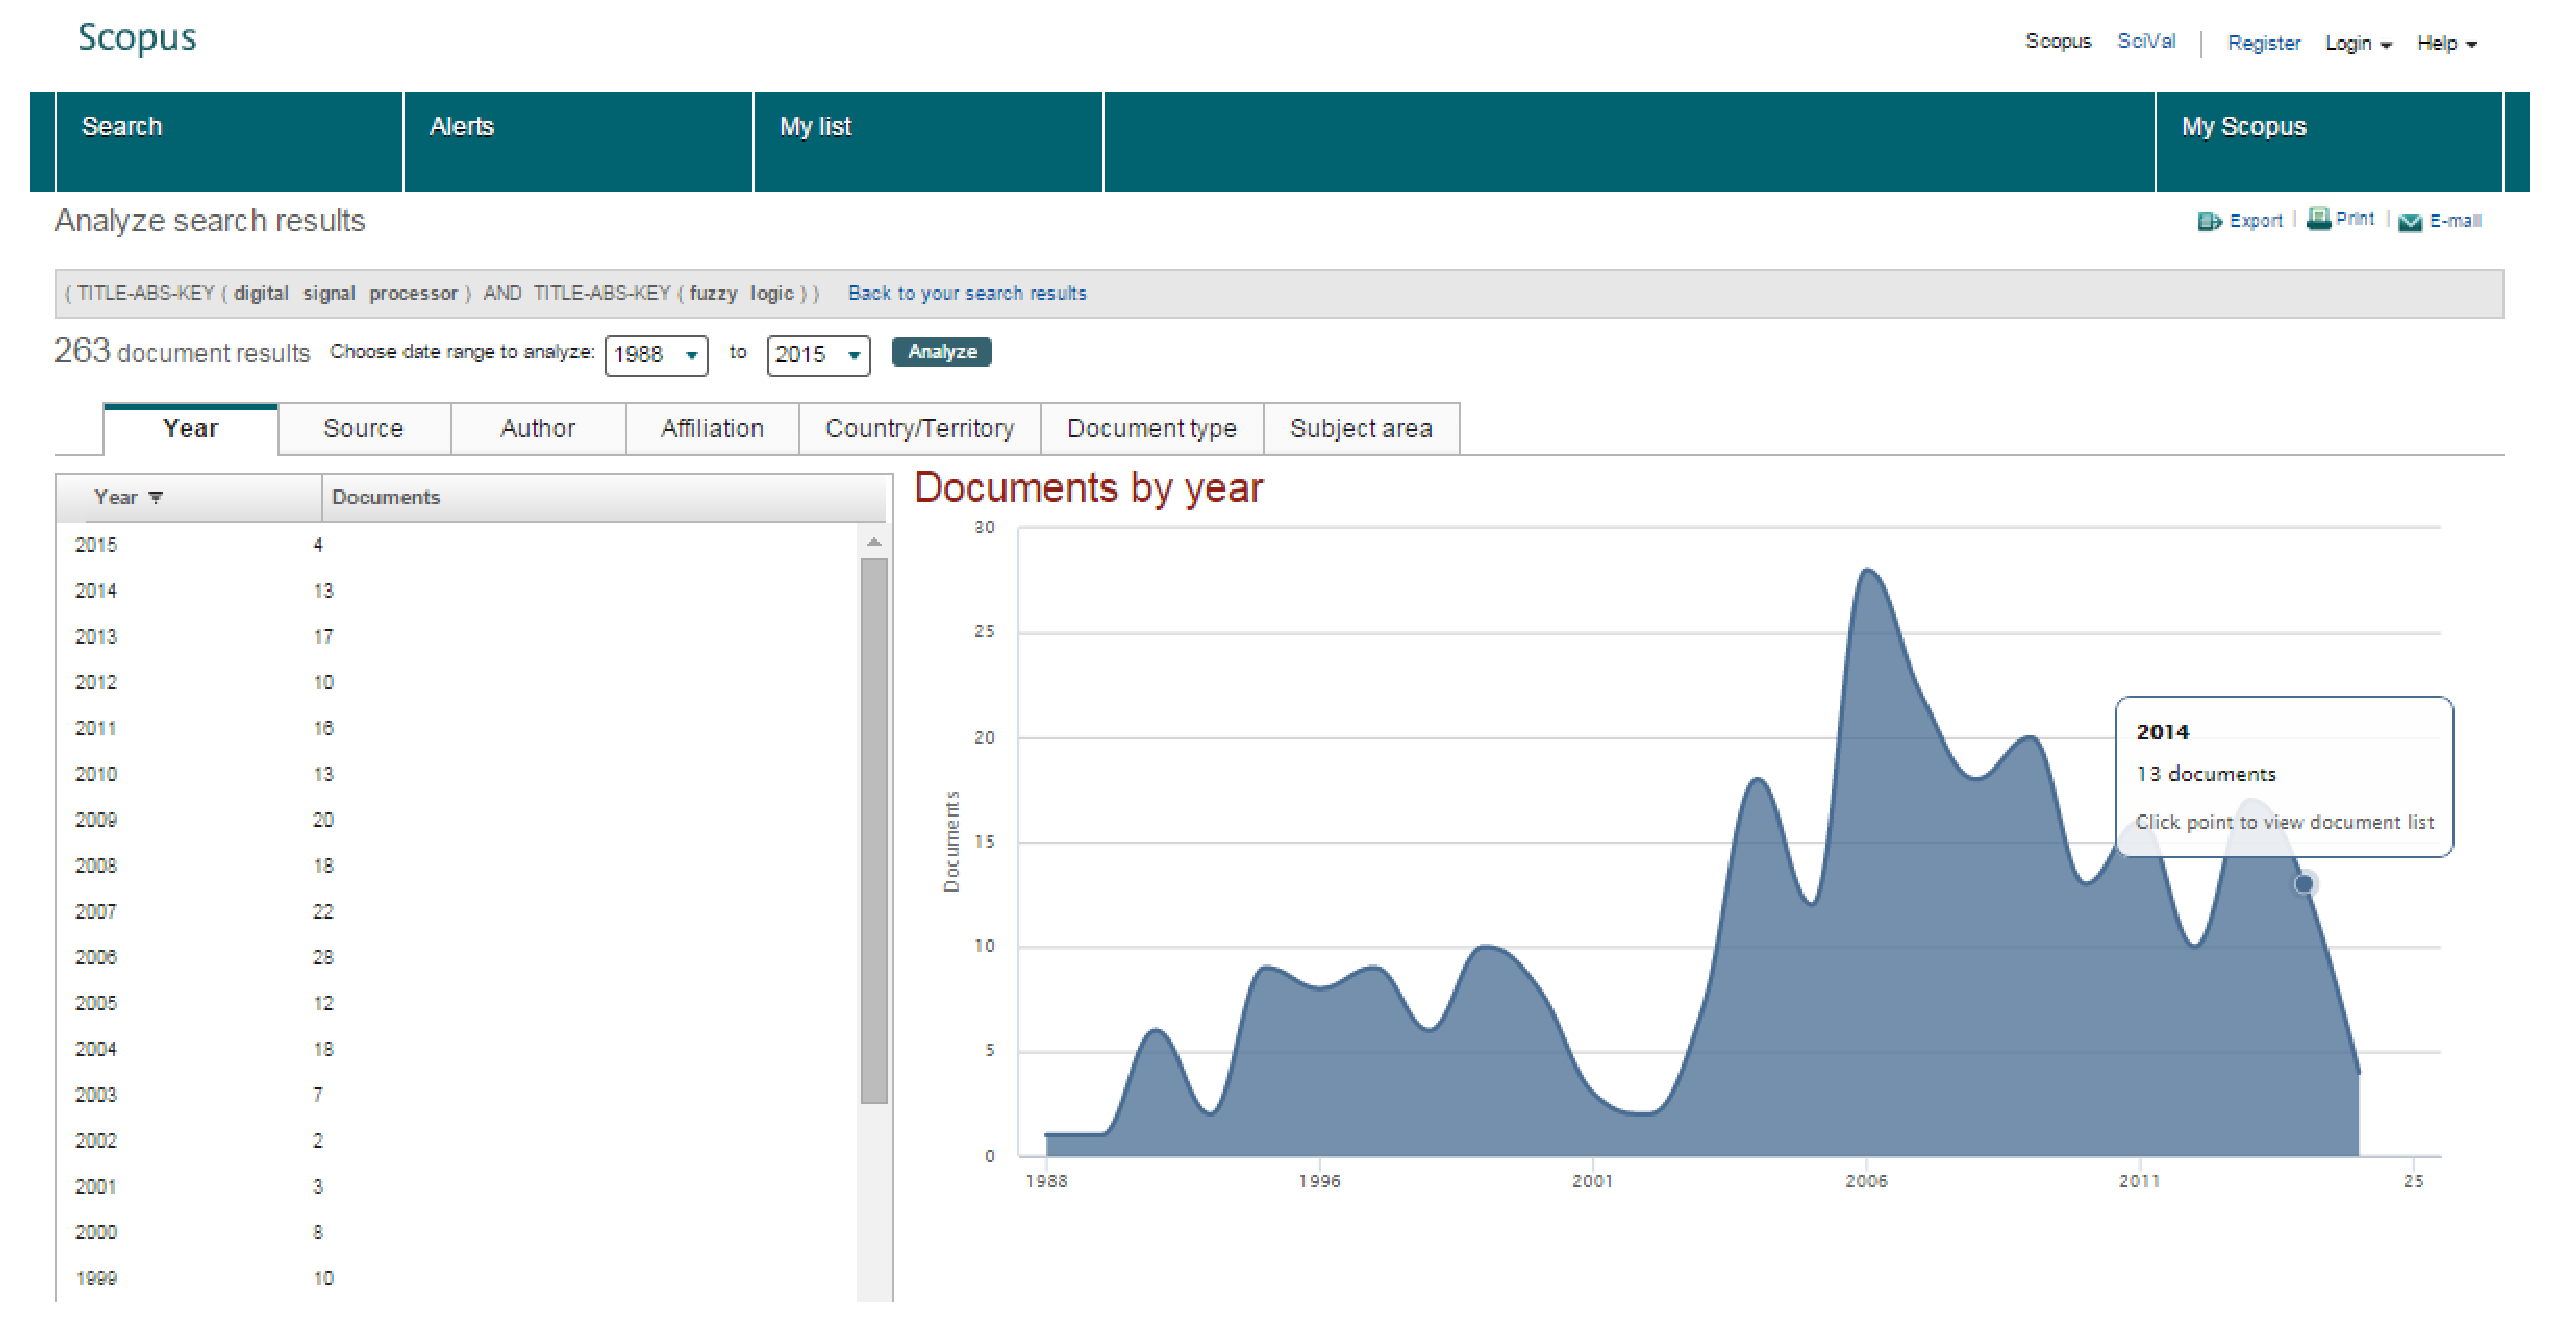
\includegraphics[width=1\linewidth]{Chapter1/chapter1/Fig3_DSP_trend}
	\caption{Literature on DSP implementation of FLCS as reported by scopus as on May 2015}
	\label{fig:Fig3_DSP}
\end{figure}

\subsection{Comparison between various Digital Platform for FLCS Implementation}
It can be seen from Figure \ref{fig:Fig2_FPGA} that FPGA have been most preferred FLCS design platform in literature  \cite{Brox2013,Adhavan2014a,Maji2014a,Messai2011,Tamukoh2007,Schrieber2015,Palakeerthi2014,Santos2014,Benzekri20146109,Islam2013}. Some FLCS architectures have also been developed over an application specific integrated circuit (ASIC) \cite{RoyChowdhury2011,Martinez-Rodriguez2015,Brox2013,Murshid2011,DaijinKim2000} attaining a speed of more than 50 MFLIPS \cite{Bosque2014b,Zavala2012,Murshid2011}. However, the design of these controllers does not make them truly reconfigurable in nature. The major disadvantage is their unavailability for field or on\hyp{}line tuning \cite{Bosque2014b,Passino2010}. It has also been observed that many of the ASIC based designs have been developed using membership function generators (MFGs). MFG circuitry can tune the membership functions (MFs) by setting some voltages on IC pins \cite{Soleimani2014,Mokarram2015} but the Rulebase remains static. To ensure field tunability, it is necessary to impart the FLCS with features that would enable users to change control parameters in run\hyp{}time. In some of the FLCS designs, the fuzzy parameters are stored in digital memory as weights \cite{Bosque2014b,Zavala2012,Kalaykov1999} to impart features of tunability. This technique permits a look-up-table based approach for fuzzy computations which reduces the computation time. However, the online reconfigurability of such system becomes difficult. This technique is well suited for application specific FLCS design where the rulebase and the parameters remain unchanged during the majority of the operation.

Though most of these designs are based on ASIC or FPGA platform, many of the designs are developed on DSP platform for its ease of implementation and reconfigurability \cite{AlNabulsi2012,Kalaykov1999,Mustafa2010,Rubaai2007,Gai2010,Uddin2007,Mohanasundaram201187,wangHuang2013,Maji2013,maji2012design}. From Figure \ref{fig:Fig3_DSP} it is evident that DSP have been also been a preferred platform for implementation of FLCS designs. However, these designs suffer from limitations on the flexibility of weight update. Recently, few RISC processors have included dedicated fuzzy instructions and have been seen to deliver a very high performance in terms of FLIPS \cite{Salapura1998,Watanabe1996,Brox2006,bookGoos2003}. These designs are summarized in Table \ref{tab:survey} where the number of inputs and outputs supported by these systems and maximum number of rules that can be evaluated by these systems is listed. However, the common limitation of many of these designs is that the control parameters can be updated only by removing these controllers from the system, rendering the plant off\hyp{}line. Some of the works have reported to update parameters on\hyp{}line through complex learning processes \cite{Munoz-Salinas2008,Alcala2006,Bandyopadhyay2001a,Boubertakh2010,Demir2011b}. 
In the current decade, DSP based FLCS designs have been widely used in control applications\cite{Heber1997,Butt2004,Suetake2011,Uddin2006}. Over 250 DSP based fuzzy system designs have been reported in last decade according to \url{www.scopus.com}. It has been found that some of the most preferred DSP platforms for this type of design are Texas Instruments' TMS320F series DSPs\cite{Rahmani2013,Pu2014,Eskandarian2014,ElKhateb2014,Okumus2014,Hung2015}, TMS320C series DSPs\cite{Sousa1995,Mustafa2010,Uddin2006,Gai2010,Uddin2007} and dSpace DSPs\cite{MatIsa2012,Noman2013,Rafa2014,Rubaai2007,Butt2004}. The DSP platform is also found to be a preferred platform for FLCS design. 

Even though FPGA is preferred platform for implementation of FLCs compared to a programmable DSP, in this work implementation is done using a TI C6748 DSP processor.  The primary reasons for selection of the mentioned hardware include:
\begin{itemize}
	\item DSP provides efficient implementation of multiplication and accumulation (MAC) and this helps COA implementation.
	\item File handling and socket programming is an integral part of this design. These are achieved easily since the development is done using C language.
	\item This design supports high level of branching and decision making.
\end{itemize}	
Collectively, for this architecture, DSPs were judicially selected over conventional FPGAs. 

\section{Generic Fuzzy Logic Controller}
Generic fuzzy logic controller systems (G\hyp{}FLCS) are standalone and remotely tunable fuzzy logic control devices. These devices are developed on suitable hardware platforms such that they can be easily interfaced with various process plants. The major characteristic of these type of devices is that they do not require reprogramming. These devices accept fuzzy parameters from the users externally through some user interfaces or programmable pins.

\begin{table}[h!]
	\centering
	\caption{Important works on G\hyp{}FLCS}
	\label{tab:survey}
	\resizebox{0.65\textwidth}{!}{%
		\begin{tabular}{llll}
			\hline \noalign{\vskip 2mm}
			Year & \begin{tabular}[c]{@{}l@{}}Speed\\ (in FLIPS)\end{tabular} & Platform & Features \\ \noalign{\vskip 2mm} \hline  \noalign{\vskip 2mm}
			\begin{tabular}[c]{@{}l@{}}1995\\ \cite{Miki1995}\end{tabular} & 0.63M & \begin{tabular}[c]{@{}l@{}}BiCMOS\\ 2$\mu$m\end{tabular} & \begin{tabular}[c]{@{}l@{}}Output MFs: Singleton (7)\\ I/O: 5 bit\\ Input MFs: 11\\ Overlaps: 2\\ Rules Evaluated: 4 per IC\end{tabular} \\ \noalign{\vskip 3mm}  
			\begin{tabular}[c]{@{}l@{}}1996\\ \cite{Watanabe1996}\end{tabular} & 48-122 & \begin{tabular}[c]{@{}l@{}}R3000A \\ RISC\\ Fuzzy \\ Processor\end{tabular} & \begin{tabular}[c]{@{}l@{}}Output MFs: -\\ I/O: -\\ Input MFs: \\ Overlaps: 2\\ Rules Evaluated: 51\end{tabular} \\ \noalign{\vskip 3mm}
			\begin{tabular}[c]{@{}l@{}}2005\\ \cite{Amirkhanzadeh2005}\end{tabular} & 15.87M & \begin{tabular}[c]{@{}l@{}}CMOS\\ 0.35 $\mu$m\end{tabular} & \begin{tabular}[c]{@{}l@{}}Output MFs: Singleton (7)\\ I/O: 2-1\\ Input MFs: 3\\ Overlaps: 2\\ Rules Evaluated: 9\end{tabular} \\ \noalign{\vskip 3mm}
			\begin{tabular}[c]{@{}l@{}}2007\\ \cite{Yosefi2007}\end{tabular} & 16.6M & \begin{tabular}[c]{@{}l@{}}CMOS\\ 0.35 $\mu$ m\end{tabular} & \begin{tabular}[c]{@{}l@{}}Output MFs: Singleton (7)\\ I/O: 2-1\\ Input MFs: 4\\ Overlaps: -\\ Rules Evaluated: 16\end{tabular} \\ \noalign{\vskip 3mm}
			\begin{tabular}[c]{@{}l@{}}2007-2008\\ \cite{Gonzalez2007}\\ \cite{Olivas2008}\end{tabular} & 5.5K & FPGA & \begin{tabular}[c]{@{}l@{}}Output MFs: Singleton (5)\\ I/O: 2-1\\ Input MFs: 8\\ Overlaps: -\\ Rules Evaluated: 64\end{tabular} \\ \noalign{\vskip 3mm}
			\begin{tabular}[c]{@{}l@{}}2010\\ \cite{Fu2010}\end{tabular} & 11K & FPGA & \begin{tabular}[c]{@{}l@{}}Output MFs: - (5)\\ I/O: 2-1\\ Input MFs: 5\\ Overlaps: 2\\ Rules Evaluated: 25\end{tabular} \\ \noalign{\vskip 3mm}
			\begin{tabular}[c]{@{}l@{}}2011\\ \cite{Yosefi2011}\end{tabular} & 16.6M & CMOS & \begin{tabular}[c]{@{}l@{}}Output MFs: Singleton (7)\\ I/O: 2-1\\ Input MFs: 4\\ Overlaps: 2\\ Rules Evaluated:16\end{tabular} \\ \noalign{\vskip 3mm} 
			\begin{tabular}[c]{@{}l@{}}2014\\ \cite{Soleimani2014}\end{tabular} & 15M & \begin{tabular}[c]{@{}l@{}}CMOS\\ 0.35 $\mu$m\end{tabular} & \begin{tabular}[c]{@{}l@{}}Output MFs: Singleton(7) \\ I/O: 2-1\\ Input MFs: 5\\ Overlaps: 2\\ Rules Evaluated:25\end{tabular} \\ \noalign{\vskip 3mm}
			\begin{tabular}[c]{@{}l@{}}2015\\ \cite{Mokarram2015}\end{tabular} & NA & \begin{tabular}[c]{@{}l@{}}CMOS\\ 0.35 $\mu$m\end{tabular} & \begin{tabular}[c]{@{}l@{}}Output MFs: Singleton \\ I/O: 2-1\\ Input MFs: 4\\ Overlaps: 2\\ Rules Evaluated:16\end{tabular} \\ \noalign{\vskip 2mm} \hline
		\end{tabular}
	}
\end{table}

G\hyp{}FLCS designs are mostly crippled by their operational speed and hence they are generally forced to operate under reduced functionalities. Some of the prime G\hyp{}FLCS designs on various platforms have been surveyed and tabulated in Table \ref{tab:survey}. The table also lists the fuzzy parameters reported in these designs. The following observations have been summed up after analyzing these designs. 
\begin{itemize}
	\item It can be observed, that majority of these designs use singleton MFs at the output to reduce computational complexity. Centroid of area (COA) method when applied to singleton, which is commonly known as weighted average defuzzification method yields far low computational complexity. However, unlike COA, weighted average does not compute the area under the curve produced from the fuzzy outputs \cite{Ross2010}. It can be observed that COA presented in eq. \eqref{eq:COA_origin} 
		\begin{equation} \label{eq:COA_origin}
		Y^* = \frac{{\int {{\mu _c}(y)ydy} }}{{\int {{\mu _c}(y)dy} }}
		\end{equation}
	can reduced to weighted average	as depicted in eq. \eqref{eq:wtAvg}.
	\begin{equation}\label{eq:wtAvg}
	{Y^*} = \frac{{\sum {{\mu _c}(y) \cdot y} }}{{\sum {{\mu _c}(y)} }}
	\end{equation}
	where $ Y^* $ represents the crisp output computed from output fuzzy set $ {\mu _c}(y) $ and output support membership function value $ y $.
	\item These designs uses a stringent rule reduction technique where only two overlapping memberships have been considered.
	\item These systems evaluate very few rules to improve computational speed. The reduction in the number of rules with only two overlapping membership functions does not provide desired performance in terms of accuracy of the system for many applications.
	\item In general, these systems cannot be remotely tuned. Some of these devices have MFGs for tuning MFs but the Rulebase remains static and the performance is limited to two inputs. 
\end{itemize} 	
These limitations motivate research in soft\hyp{}core generic FLC devices on programmable hardware where multifarious control over the system can be obtained by varying different control parameters with modest computational complexity.

\section{Problem Statement}
The limitations of the existing G\hyp{}FLCS designs, as defined in Table \ref{tab:survey}, motivated the research in developing a soft\hyp{}core G\hyp{}FLCS device on programmable DSP hardware with two level tuning where multifarious control over the system can be obtained with modest computational complexity. However, this design is extremely challenging owing to following conditions.
\begin{itemize}
\item Since the proposed design is expected to command a large number of fuzzy parameters; it is imperative to develop an interactive interface for guiding users to input fuzzy parameters.
\item It is also a known fact that human beings are prone to make errors while handling large data. Therefore, an automated system has to be deployed which will extract coarse fuzzy parameters from a large input\hyp{}output dataset.
\item The significant challenges in designing such a system lies in managing an exponentially growing rulebase. Therefore, development of a suitable rule reduction technique is required which will generate a desired output consuming minimum cycle time.
\item It has been discussed previously that defuzzification module in FLCS using COA technique is computationally quite expensive. A desirable COA scheme with low computation time is essential to achieving a dependable system cycle time that is relevant to the majority of control applications.
\end{itemize}

\section{Outline of Thesis}
The thesis is presented in 6 chapters. Following this chapter on introduction, the remaining thesis is organized as under:
This thesis is organized as follows:
\begin{itemize}
	\item Chapter 2 presents a mathematical model of the generic fuzzy logic controller and describes the proposed MT\hyp{}FRHC rule reduction technique. A vertices based centroid of area computation algorithm for defuzzification is also proposed.
	\item Chapter 3 explains the design architecture and develops the backbone of the proposed the G\hyp{}FLCS. The proposed architecture includes a web based user interface (WebUI) for users to program fuzzy parameters in  the GFLCS, a genetic algorithm based fuzzy parameter extraction scheme and a fuzzy framework.
	\item Chapter 4 implements the concepts developed in Chapter 2 and 3 in optimized C code and realizes the proposed G\hyp{}FLCS on a C6748 DSP processor. Applicability and performance analysis of the G\hyp{}FLCS is analyzed.
	\item In Chapter 5, the proposed G\hyp{}FLCS is used to control the radial position of plasma in Aditya Tokamak Fusion Test Reactor (TFTR). The GA based fuzzy parameter extraction process is used to obtain FCP for the control problem. This FCP is used to control the plasma position in the Aditya TFTR Simulink model and the same is compared to some of the previously developed systems.
	\item Finally the research work is concluded in chapter 6 and the scope of future work is explained briefly. The limitations and the scope for future work of this research are also elaborated in this chapter.
\end{itemize}

